\documentclass[12pt, a4paper]{article}
\usepackage[german]{babel}
\usepackage{graphicx}

\title{Einführung und Digitalisierung eines neuen Geschäftsprozesses - Sichtprüfung und Inventur von EFTs}
\author{Kilian Schlosser}
\date{Sommersemester 2023}

\begin{document}


\maketitle


\tableofcontents
\newpage

\section{Einleitung}

Diese Arbeit beschäftigt sich mit der Einführung eines neuen Geschäftsprozesses zur Inventarisierung und Sichtprüfung von Electronic Funds Transfers (EFTs), also den Bezahlterminals 
an den Kassen. 
Das Ziel besteht darin, den bestehenden manuellen Prozess zu optimieren und durch eine digitale Lösung zu ersetzen. Diese Einleitung gibt einen Überblick über die 
Aufgabenstellung, die Einbettung des Themas in ein größeres Umfeld und bietet einen Ausblick auf die weiteren Kapitel dieser Arbeit.

Die Motivation dahinter stammt aus einem Projekt der tegut... gute Lebensmittel GmbH \& Co. KG (nachfolgend nur kurz tegut... genannt) zur Verschlüsselung der Übertragung von
Kreditkartendaten vom Bezahlterminal zum Zahlungsdienstleister. Um die Firmware einsetzen zu können, die diese Verschlüsselung ermöglicht, muss tegut... eine höhere Stufe der 
"Payment Card Industry Data Security Standard"-Zertifizierung (PCI-DSS) als bislang erreichen. Um dieser gerecht zu werden, muss unter Anderem eine laufende Inventur und
Sichtprüfung aller aktiv eingesetzten EFTs gewährleistet sein.
Die zunehmende Digitalisierung und Automatisierung von Geschäftsprozessen hat in den letzten Jahren zu großen Verbesserungen in Effizienz und Genauigkeit in der Verwaltung geführt.
Die Inventarisierung von EFTs stellt jedoch weiterhin eine Herausforderung dar, da der aktuelle Prozess manuell und teilweise papierbasiert ist sowie nicht regelmäßig 
durchgeführt wird. 
Um diese Schwachstellen zu beheben, wird in dieser Arbeit ein neuer Geschäftsprozess eingeführt, der die Vorteile der Digitalisierung nutzt. 

Die Arbeit ist in mehrere Kapitel unterteilt, die jeweils verschiedene Aspekte der Problematik behandeln. Im zweiten Kapitel wird die Planungsphase näher beschrieben, 
in der der IST-Prozess analysiert und Schwachstellen identifiziert werden. Dabei wird auch die Wahl der Bizagi-Plattform als Lösung zur Digitalisierung des Prozesses erläutert. 
Das dritte Kapitel widmet sich der Modellierung des SOLL-Prozesses und zeigt auf, wie die Inventarisierung und Sichtprüfung der EFTs digitalisiert und automatisiert werden 
können.

Im vierten Kapitel wird die Einführung und Abstimmung des neuen Geschäftsprozesses diskutiert. Es werden die verschiedenen Stakeholder einbezogen und deren Bedürfnisse 
berücksichtigt, um eine reibungslose Implementierung zu gewährleisten.

Abschließend werden die wichtigsten Erkenntnisse zusammengefasst und ein Ausblick auf mögliche zukünftige Entwicklungen gegeben.

\section{Planungsphase}

Eine entscheidende Phase vor der eigentlichen Implementierung des neuen Geschäftsprozesses war die Planungsphase. Hier wurden grundlegende Überlegungen und Entscheidungen 
getroffen, die die Basis für die spätere Umsetzung bildeten. Ein Hauptaugenmerk lag dabei auf der Wahl des optimalen Endgeräts für den Prozess.
Zusätzlich besteht sie aus einer detaillierten Analyse des IST-Prozesses, Identifikation der Schwachstellen und einer gezielten Lösungssuche.

\subsection{Analyse des IST-Prozesses}

Eine detaillierte Aufnahme des bestehenden Prozesses war essentiell, um die aktuellen Abläufe, Verantwortlichkeiten und Tools zu verstehen. Hierbei wurden folgende Punkte 
festgestellt:
\begin{itemize}
\item Die EFTs wurden bei Lieferung manuell in Listen erfasst und mit Inventaraufklebern versehen.
\item Anschließend wurde die Liste in die Content Management Database (CMDB) importiert.
\item Bei Auslieferung an eine Filiale wurde die Filial- und Kassennummer nachgetragen.
\item Die Abläufe waren nicht fest definiert.
\end{itemize}
Einen Prozess zur laufenden Inventur oder einer Sichtprüfung gab es bislang nicht.

\subsection{Identifikation von Schwachstellen}

Die Analyse hat mehrere Schwachstellen des IST-Prozesses offengelegt:
\begin{itemize}
\item Zeitaufwand: Der manuelle Prozess ist zeitaufwändig und erfordert mehrere Mitarbeiter.
\item Nachverfolgbarkeit: Ohne eine regelmäßige Inventur ist es schwierig, einen Überblick über alle EFTs zu behalten und sie nachzuverfolgen.
\item Reproduzierbarkeit: Ohne festgeschriebene Abläufe kann der Prozess nicht jedes Mal korrekt reproduziert werden.
\end{itemize}
Der Prozess zur Aufnahme der EFTs in das Inventar, ist ein Standardprozess für alle neue Hardware bei tegut... . Diesen Prozess neu zu gestalten ist nicht Bestandteil dieser
Arbeit und wird bei tegut... bereits in einem separatem Projekt bearbeitet.

\subsection{Wahl der Bizagi-Plattform}

Nach einer gründlichen Marktanalyse wurde die Bizagi-Plattform schon vor einigen Jahren von tegut... als ideale Lösung zur Digitalisierung von Geschäftsprozessen gewählt. 
Einige Vorteile dieser Plattform sind:
\begin{itemize}
\item Benutzerfreundlichkeit: Die Plattform bietet eine intuitive Benutzeroberfläche, die den Übergang von einem manuellen zu einem digitalen Prozess erleichtert.
\item Flexibilität: Die Plattform ermöglicht es, den Prozess nach Bedarf anzupassen und zu erweitern.
\end{itemize}
Die Implementierung des Prozesses mit Hilfe der Bizagi-Plattform wird im nächsten Kapitel näher erläutert.

\subsection{Mobil vs. Stationär: Die Wahl des Endgeräts}

Die Verwendung eines geeigneten Endgeräts ist entscheidend für den Erfolg des digitalisierten Prozesses. Insbesondere ging es darum, ob moderne MDEs oder herkömmliche PCs 
eingesetzt werden sollten.

\subsubsection{Mobile Datenerfassungsgeräte (MDEs)}

\textbf{Vorteile:}
\begin{itemize}
\item \textit{Mobilität:} MDEs können überall hin mitgenommen werden, was gerade bei der Erfassung von EFTs vor Ort sehr nützlich ist.
\item \textit{Echtzeit-Erfassung:} Daten können sofort vor Ort eingegeben und übertragen werden.
\item \textit{Barcodescanner und Kamera:} Die MDEs sind mit Barcodescannern und Kameras ausgestattet, was die Datenerfassung erleichtert.
\end{itemize}

\textbf{Nachteile:}
\begin{itemize}
\item \textit{Begrenzte Bildschirmgröße:} Die Erfassung komplexer Daten kann schwieriger sein als auf einem PC.
\end{itemize}

\subsubsection{Personal Computer (PC)}

\textbf{Vorteile:}
\begin{itemize}
\item \textit{Größerer Bildschirm:} Dies ermöglicht eine übersichtlichere Darstellung und leichtere Eingabe komplexer Daten.
\item \textit{Leistungsfähigkeit:} PCs können komplexe Aufgaben schneller verarbeiten.
\item \textit{Standardisierung:} PCs sind bereits in den Büros der Filialen vorhanden und die Mitarbeiter sind mit ihrer Bedienung vertraut.
\end{itemize}

\textbf{Nachteile:}
\begin{itemize}
\item \textit{Mobilität:} PCs sind stationär und nicht für den mobilen Einsatz vor Ort geeignet. Das erhöht die Fehlerquote bei der Übertragung von komplexen Daten,
wie Inventar- oder Seriennummern.
\end{itemize}

\subsubsection{Entscheidung}
Nach sorgfältiger Abwägung aller Vor- und Nachteile beider Lösungen wurde in Absprache mit dem Enterprise Architekten der tegut...-Informationstechnologie entschieden, 
den Prozess zunächst für den PC zu modellieren. Diese Entscheidung wurde maßgeblich von der Tatsache beeinflusst, dass noch nicht alle Filialen die neuen, Android-betriebenen 
MDEs verwenden. Zudem legt der Enterprise Architekt Wert darauf, dass die MDEs als Plattform so isoliert wie möglich betrieben werden. \cite{Schlosser_Ehm_2023} Außerdem haben alle Filialleiter ein Notebook,
das zur Durchführung der Inventur und Sichtprüfung benutzt werden kann. Zusätzlich hilft die Verwendung von Notebooks, den Nachteil der geringeren Mobilität 
eines stationären PCs zu umgehen, was insbesondere in den Filialräumlichkeiten von Vorteil ist, da die Filialleiter die Möglichkeit haben, sich während der Durchführung 
der Inventur und Sichtprüfung frei zu bewegen.


\section{Modellierung des SOLL-Prozesses}

Nachdem die Schwachstellen des IST-Prozesses identifiziert und die Bizagi-Plattform als Lösung ausgewählt wurde, folgt nun die Modellierung des gewünschten (SOLL) Prozesses. 
Dieser Abschnitt beschreibt die Schritte und Überlegungen, die in diese Phase eingeflossen sind.

\subsection{Ziele des SOLL-Prozesses}

Zunächst wurden die Hauptziele für den neuen Prozess definiert:
\begin{itemize}
\item Minimierung des manuellen Aufwands durch Automatisierung.
\item Erhöhung der Transparenz und Nachverfolgbarkeit von EFTs.
\item Sicherstellung der Datenkonsistenz und -integrität.
\item Erfüllung des PCI-DSS Standards.
\end{itemize}


\subsection{Modellierung des SOLL-Prozesses mit Bizagi}

Bizagi ist eine renommierte Plattform für die Geschäftsprozessmodellierung und -automatisierung. Die Software bietet verschiedene Werkzeuge zur Darstellung, 
Optimierung und Digitalisierung von Geschäftsprozessen. In diesem Teilabschnitt wird erläutert, wie Bizagi zur Modellierung des SOLL-Prozesses verwendet wurde und welche 
Vorteile die Plattform in diesem Kontext bietet.

\subsubsection{Möglichkeiten von Bizagi}

Bizagi bietet eine Vielzahl von Funktionen, die den gesamten Lebenszyklus eines Geschäftsprozesses abdecken:

\begin{itemize}
\item \textit{Drag-and-Drop-Prozessmodellierung:} Die intuitive Benutzeroberfläche ermöglicht es, Geschäftsprozesse einfach durch Drag-and-Drop zu modellieren, 
wodurch kein technisches Vorwissen erforderlich ist.
\item \textit{Integrierte Datenbank:} Bizagi ermöglicht eine nahtlose Integration mit bestehenden Datenbanken und Systemen.
\item \textit{Formular-Designer:} Mit dem integrierten Formular-Designer können Eingabemasken für Benutzer erstellt werden, um Daten effizient zu erfassen.
\item \textit{Automatisierung und Ausführung:} Einmal modellierte Prozesse können automatisiert und direkt in Bizagi ausgeführt werden.
\item \textit{Berichterstattung und Analyse:} Bizagi bietet leistungsstarke Analysetools, um den Fortschritt und die Leistung von Geschäftsprozessen zu überwachen.
\end{itemize}

\subsubsection{Schritte zur Digitalisierung des Prozesses}

\begin{enumerate}
\item \textit{Analyse des IST-Prozesses:} Vor Beginn der eigentlichen Modellierung wurde der aktuelle, manuelle Prozess analysiert, um Schwachstellen und 
Verbesserungspotenziale zu identifizieren.
\item \textit{Prozessmodellierung:} Mit Hilfe des Bizagi Modelers wurde der SOLL-Prozess Schritt für Schritt modelliert.
\item \textit{Formulargestaltung:} Für den modellierten Prozess wurden entsprechende Eingabemasken mit dem Formular-Designer erstellt.
\end{enumerate}


Durch die Nutzung von Bizagi konnte der neue Geschäftsprozess effizient modelliert, optimiert und schließlich digitalisiert werden. Dabei hat sich besonders der 
Formular-Designer als wertvolles Werkzeug herausgestellt, da er eine einfache und intuitive Erfassung der benötigten Daten ermöglicht.

\subsubsection{Erstellung des Datenmodells}
Um das Datenmodell zu erstellen, wurde ein Export eines EFT-Eintrags aus der CMDB als Grundlage genommen. Bizagi bietet die Möglichkeit, ein Datenmodell auf Grundlage einer 
Excel-Datei zu erstellen und diese Felder mit Eingabemasken aus dem Formulardesigner zu verknüpfen. Um den Anforderungen des PCI-DSS Standards gerecht zu werden, mussten in der
CMDB auch einige Felder hinzugefügt werden, um die Überprüfungskriterien mit aufzunehmen. Das spiegelt sich auch im Datenmodell wieder.
Folgende Kriterien müssen überprüft  werden:

\begin{itemize}
    \item Defektes Gehäuse
    \item Anschluss externer Module
    \item Unversehrtheit von Siegeln und Plomben
    \item Unversehrtheit des Inventaraufklebers und der Terminal-ID
    \item Sonstige Auffälligkeiten (z. B. lose Kabel, herausragende Drähte, neue Aufkleber oder andere Markierungen etc.)
\end{itemize}

\cite{Würz_Gebauer_2022}

Schlussendlich sieht das Datenmodell aus, wie in \ref{fig:data-model} abgebildet.
Damit die Daten in Bizagi aktuell sind, wird aus dem ServiceNow regelmäßig ein Export der Einträge aller EFT-Geräte erstellt. Momentan muss diese Export-Liste noch händisch
nach Bizagi importiert werden. Da das aber ein Aufwand von nur wenigen Minuten für den zuständigen Mitarbeiter ist, wurde vorerst darauf verzichtet eine komplett automatisierte 
Lösung zu entwickeln.

\begin{figure}
    \centering
    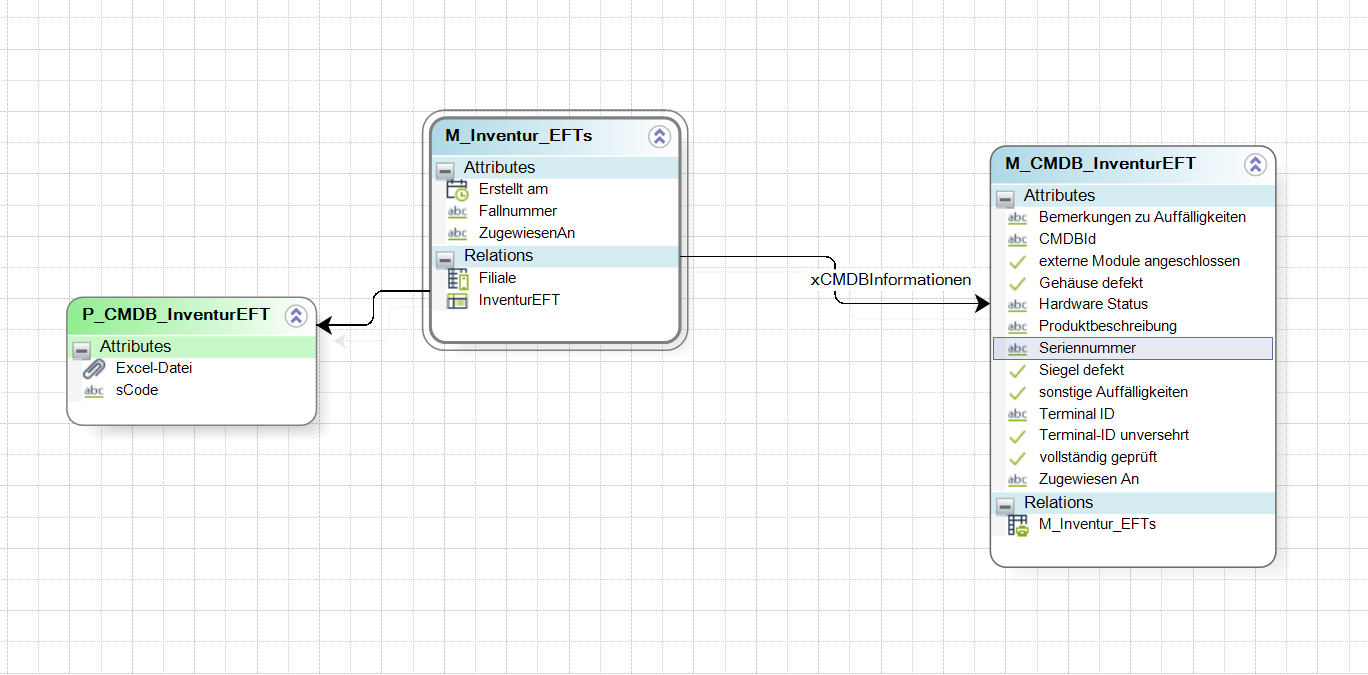
\includegraphics[width=\textwidth]{images/data-model.png}
    \caption{Screenshot des Datenmodells in Bizagi}
    \label{fig:data-model}
\end{figure}
\newpage

\subsection{Hauptkomponenten und Abläufe}

Mit Hilfe der Bizagi-Plattform wurden die folgenden Hauptkomponenten und Abläufe für den SOLL-Prozess modelliert:

\begin{itemize}
\item Integration mit CMDB: Obwohl eine zentrale Datenbank (CMDB) bereits existiert und mit ServiceNow betrieben wird, hat die starke Anpassung von ServiceNow seitens tegut... 
die direkte Integration mit Bizagi erschwert. Daher erfolgt die Aktualisierung der CMDB indirekt.
\item Benachrichtigungssystem: Bei Abweichungen oder Anmerkungen werden die Mitarbeiter der entsprechenden Fachabteilung informiert. Dies ermöglicht es ihnen, die 
CMDB manuell über ServiceNow zu aktualisieren und dem Vorfall nachzugehen.
\item Inventur: Die Benutzer bekommen die aktuellen Daten zu den einzelnen EFTs der entsprechenden Filiale aus der CMDB zum Abgleich zur Verfügung gestellt
\item Sichtprüfung: In der Maske zum Abgleich der Daten können die Nutzer ebenfalls eintragen, ob das EFT in irgendeiner Art und Weise manipuliert wurde oder ob es Auffälligkeiten gibt. 
\end{itemize}

\begin{figure}
    \centering
    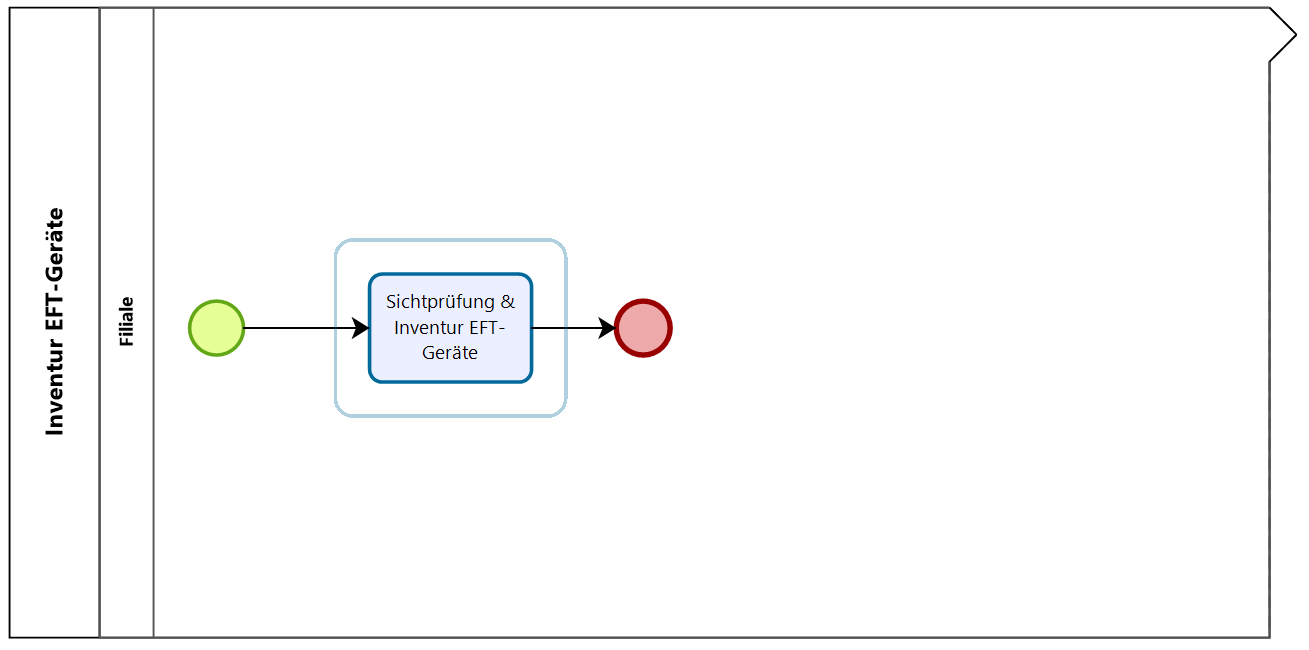
\includegraphics[width=\textwidth]{images/process.png}
    \caption{Screenshot des modellierten SOLL-Prozesses in Bizagi}
    \label{fig:soll_process}
\end{figure}

Wie in Abbildung \ref{fig:soll_process} zu sehen ist, ist das Prozessmodell in seiner Grundstruktur sehr einfach. Nach intensiver Überlegung wurde entschieden, 
sämtliche Schritte innerhalb dieser einen Aktivität im Formular abzubilden. Dies macht das Prozessmodell auf den ersten Blick zwar etwas weniger transparent, erhöht 
jedoch die Benutzerfreundlichkeit des Formulars, da weniger häufige Wechsel zwischen verschiedenen Masken notwendig sind.

\begin{figure}
    \centering
    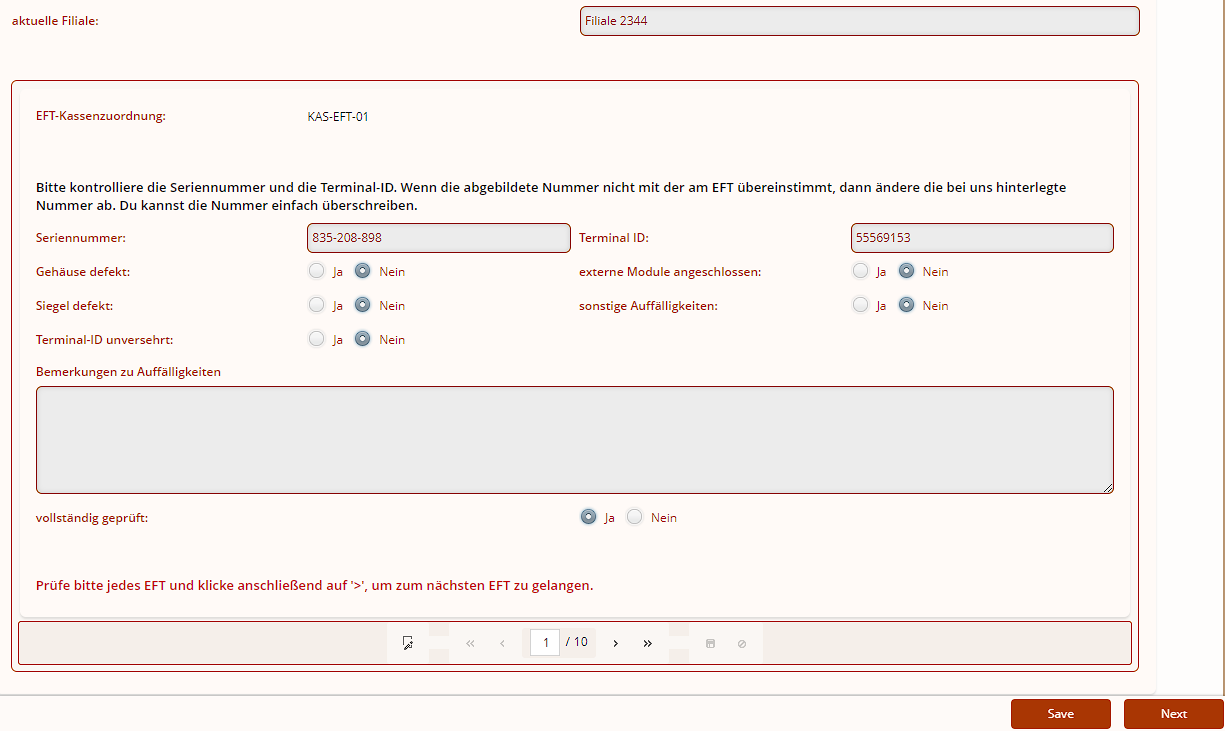
\includegraphics[width=\textwidth]{images/eingabemaske.png}
    \caption{Screenshot der Eingabemaske mit Beispieldaten}
    \label{fig:maske}
\end{figure}

Der Prozess beginnt damit, dass sich ein Mitarbeiter mit seinem Filialkonto bei der Bizagi-Cloud anmeldet. Nach erfolgreicher Anmeldung initiiert der Mitarbeiter 
einen neuen Vorgang unter der Bezeichnung \textit{Inventur EFT-Geräte}. Auf Grundlage der Anmeldedaten filtert Bizagi automatisch die für den jeweiligen Mitarbeiter zugehörigen 
EFT-Geräte aus der vorhandenen Liste heraus und stellt diese im System bereit.

Für jedes dieser EFT-Geräte wird nun in der Benutzeroberfläche eine separate Seite innerhalb der Eingabemaske generiert. Auf diesen Seiten trägt der Mitarbeiter 
die relevanten Informationen im Rahmen der Inventur und Sichtprüfung ein. Nachdem alle zugeordneten EFT-Geräte kontrolliert und die entsprechenden Informationen eingetragen 
wurden, speichert der Mitarbeiter den Vorgang ab und beendet diesen im System.

Sollten während der Kontrolle Abweichungen zwischen den erfassten Daten und den bereits vorhandenen Daten im ServiceNow festgestellt werden, wird automatisch eine 
Benachrichtigung in Form einer E-Mail an die Revisionsabteilung gesendet. Die Revisionsabteilung ist dann für die Untersuchung des Vorfalls zuständig und nimmt gegebenenfalls 
notwendige Korrekturen oder weitere Schritte vor.

\section{Einführung und Abstimmung des neuen\\ Geschäftsprozesses}

Die Implementierung eines digitalisierten Geschäftsprozesses ist eine komplexe Aufgabe, die sorgfältige Planung, Koordination und Abstimmung zwischen den verschiedenen 
Stakeholdern erfordert. Im Fall des neuen Geschäftsprozesses zur Inventarisierung und Sichtprüfung der EFTs sind die relevanten Stakeholder vor allem die Mitarbeiter 
der Revisions- und IT-Abteilung sowie die Endanwender des Prozesses in den einzelnen Filialen.


\subsection{Projektkoordination und Stakeholder-Management}

Ein effektives Projektmanagement ist essentiell, um die Einführung des neuen Geschäftsprozesses koordiniert und effizient zu gestalten. 
Um zusätzliche Arbeitslast für alle Beteiligten zu vermieden, wurde kein neues Projektteam zusammengestellt. Stattdessen hat sich das Team des übergeordneten Projekts - 
bestehend aus Vertretern der IT-Abteilung, der Revision und des Vertriebs - dieser Aufgabe angenommen. Dieses Team war verantwortlich für die Entwicklung des Projektplans, 
die Identifizierung von Meilensteinen und die kontinuierliche Überwachung des Projektfortschritts.

Die Kommunikation mit den Stakeholdern war ein zentraler Aspekt des Projektmanagements. Regelmäßige Meetings und Berichterstattungen gewährleisteten, 
dass alle Beteiligten über den Stand des Projekts informiert waren und dass ihr Feedback in die Weiterentwicklung des Prozesses einfloss. 

\subsection{Evaluierung und Anpassung}

Vor der Einführung des neuen Geschäftsprozesses war es wichtig, dessen Effektivität und Effizienz zu bewerten. Dazu wurden Feedback-Sitzungen mit den Endanwendern 
durchgeführt und Performance-Metriken analysiert. Auf Grundlage der gesammelten Daten wurden Anpassungen am Geschäftsprozess vorgenommen, um die Benutzerfreundlichkeit und 
die Prozesseffizienz weiter zu verbessern.

\subsection{Schlussfolgerung}

Die Einführung und Abstimmung des neuen Geschäftsprozesses war ein iterativer und koordinierter Prozess, der die aktive Beteiligung aller Stakeholder erforderte. 
Durch effektives Projektmanagementund kontinuierliche Evaluierung wurde ein digitalisierter Geschäftsprozess geschaffen, der die Inventarisierung 
und Sichtprüfung der EFTs effizienter und benutzerfreundlicher gestaltet.

\section{Zusammenfassung und Ausblick}

\subsection{Zusammenfassung wichtiger Erkenntnisse}
Die Einführung eines digitalisierten Geschäftsprozesses für die Inventur und Sichtprüfung der EFT-Geräte bei tegut... hat eine Reihe wichtiger Erkenntnisse hervorgebracht. 
Durch die Digitalisierung konnte eine deutliche Effizienzsteigerung erzielt und die Fehleranfälligkeit des bisher manuellen, papierbasierten Prozesses reduziert werden. 
Die Implementierung der Bizagi-Plattform hat sich als passende Lösung erwiesen, um den spezifischen Anforderungen des Unternehmens gerecht zu werden. Der Einsatz von PCs, 
unter Berücksichtigung der vorhandenen Infrastruktur und der Benutzerfreundlichkeit, erwies sich als vorteilhaft. Auch die Möglichkeit der Integration mit der bereits 
bestehenden CMDB über ServiceNow, trotz einiger initialer Herausforderungen, förderte die Schaffung eines nahtlosen Workflows. Die in dieser Arbeit durchgeführten 
Prozessoptimierungen haben somit eine solide Basis für den weiteren Ausbau der digitalen Prozesslandschaft bei tegut... geschaffen.

\subsection{Ausblick}
In zukünftigen Entwicklungsphasen sollen weitere Funktionalitäten implementiert werden, um den digitalen Inventurprozess noch effizienter und benutzerfreundlicher zu gestalten. 
Eine zentrale Erweiterung stellt die Implementierung einer automatischen Benachrichtigungsfunktion dar. Dabei sollen Filialleiter automatisch über anstehende Inventur- und 
Sichtprüfungsaufgaben informiert werden, wodurch die Planung und Koordination innerhalb der Filialen weiter verbessert wird. 

Ein weiteres wesentliches Feature ist der automatische Datenimport in Bizagi. Dies würde die manuelle Dateneingabe weiter reduzieren und könnte durch eine direkte 
Anbindung an bestehende Systeme realisiert werden. Darüber hinaus könnten weitere Anpassungen und Optimierungen an den Eingabemasken und der Benutzeroberfläche vorgenommen 
werden, um die Usability kontinuierlich zu verbessern.

Die vorgenommene Digitalisierung des Inventurprozesses markiert einen wichtigen Schritt in Richtung einer umfassenderen Digitalisierungsstrategie bei tegut... und legt den 
Grundstein für die Realisierung weiterer Digitalisierungsprojekte. Durch kontinuierliche Verbesserungen und Erweiterungen des Systems kann tegut... seine Position in einem 
digitalisierten und effizienten Einzelhandelsumfeld weiter festigen und ausbauen.

\section*{Selbsständigkeitserklärung}
Ich erkläre hiermit, dass ich die vorliegende Hausarbeit ohne fremde Hilfe verfasst und nur die im Literaturverzeichnis angegebenen Quellen verwendet habe.\\

Datum: 30.09.2023

\newpage
\bibliography{bib}
\bibliographystyle{abbrvdin}

\end{document}
